\documentclass[12pt,letterpaper,reqno]{amsart}
\usepackage{enumerate}
\usepackage[shortlabels]{enumitem}
\usepackage{graphicx}
\usepackage{amssymb}
\usepackage[normalem]{ulem}
\usepackage{titlesec,bbm, hyperref}
\usepackage{spverbatim} 
\usepackage{esvect}
\usepackage{geometry}
\usepackage{caption}
\usepackage{subcaption}
\geometry{letterpaper, portrait, margin=1in}

\newcommand{\R}{\mathbb R}
\newcommand{\Q}{\mathbb Q}

\begin{document}

\thispagestyle{empty}
\centerline{\Large Math 677 Homework 2}
\centerline{Sumanth Ravipati}
\centerline{9/12/2018}
\vspace{.25in}

\begin{enumerate}
\item[(4)]
\begin{flushleft}
Consider the nonlinear oscillator system

$$\dot{x} = y$$
$$\dot{y} = -f(x)$$

with a Lipschitz continuous function $f : \R \rightarrow \R$. Let $F : \R \rightarrow \R$ be any antiderivative of $f$, and define $H(x,y) = y^2/2 + F(x)$.
\newline
\begin{enumerate}
    \item
    \begin{flushleft}
    Show that if $\lambda : I \rightarrow \R^2$ is any solution of the nonlinear oscillator system., then $H(\lambda(t)) =$ const for all $t \in I$.
    \newline
    
    If $\lambda(t)$ is a solution to the nonlinear oscillator system, we get:
    $$\frac{dH}{dt} = \frac{2y}{2}\cdot \frac{dy}{dt} + \frac{dF(x)}{dt}\cdot \frac{dx}{dt} = y\cdot \dot{y} + f(x)\cdot \dot{x} = y(-f(x)) + y(f(x)) = 0 \, \forall t \in I$$
    Therefore, $H(\lambda(t))$ is constant for all $t \in I$. Furthermore, we can say that the system is Hamiltonian since $\dot{H(x,y)} = 0$ and since:
    $$\frac{dx}{dt} = \frac{\partial{H}}{\partial{y}}$$
    $$\frac{dy}{dt} = -\frac{\partial{H}}{\partial{x}}$$
    \end{flushleft}
    \vspace{.15in}
    \item
    \begin{flushleft}
    Describe how the result of (a) can be used to find the phase portraits of the nonlinear oscillator system.
    \newline
    
    Since we have shown that the system is Hamiltonian, and that $H$ is constant for any given solution $\lambda(t)$, the phase portraits can be determined by plotting the solutions curves of the equation $H(x,y) = C$ for all possible values of the constant $C$. These solutions can be graphed on the plane with axes $x(t)$ and $y(t)$.
    \end{flushleft}
\end{enumerate}
\end{flushleft}
\newpage
\item[(5)]
\begin{flushleft}
Consider again the nonlinear oscillator system

$$\dot{x} = y$$
$$\dot{y} = -f(x)$$
\newline
For each of the following functions $f$, sketch the phase portrait of this system as precisely as possible. What types of orbits do you see?
\newline

For each of the figures below, the ones on the left are the contour plots, which are solutions to the equation $H(x,y) = C$ for a wide range of possible values for the constant $C$. The figures on the right are the actual phase portrait generated by Mathematica, and even depicts the flow of each curve through time.
\newline

\begin{enumerate}
    \item
    \begin{flushleft}
    $f(x) = 1 - x^2$
    \newline
    $$F(x) = \int f(x)dx = x - \frac{x^3}{3} + C$$
    $$H(x,y) = \frac{y^2}{2} + F(x) = \frac{y^2}{2} + x - \frac{x^3}{3} = C$$
    \end{flushleft}
    
    \begin{figure}[h]
    \centering
    \begin{subfigure}{.5\textwidth}
      \centering
      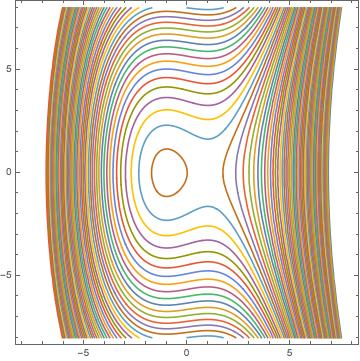
\includegraphics[width=.8\linewidth]{./ContourPlotA.jpeg}
      \caption*{eqns = Table[$\frac{y^2}{2} + x - \frac{x^3}{3} == n$, \{n, -100, 100, 2\}];}
      \caption*{ContourPlot[Evaluate@eqns, \{x, -8, 8\}, \{y, -8, 8\}]}
    \end{subfigure}%
    \begin{subfigure}{.5\textwidth}
      \centering
      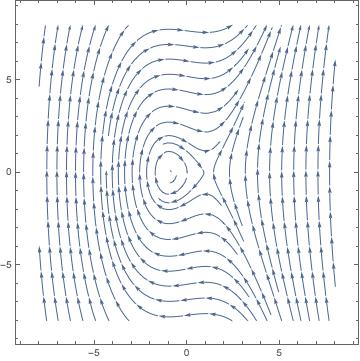
\includegraphics[width=.8\linewidth]{./StreamPlotA.jpeg}
      \caption*{StreamPlot[{$y$, $x^2 - 1$}, {x, -8, 8}, {y, -8, 8}]}
    \end{subfigure}
    \end{figure}
    
    \begin{flushleft}
    There seem to be stable, homoclinic orbits that form circles near the origin as well as saddle, hetroclinic orbits that travel away from the origin through out this phase portrait.
    \end{flushleft}
    
    \newpage
    \item
    \begin{flushleft}
    $f(x) = x - x^3$
    \newline
    $$F(x) = \int f(x)dx = \frac{x^2}{2} - \frac{x^4}{4} + C$$
    $$H(x,y) = \frac{y^2}{2} + F(x) = \frac{y^2}{2} + \frac{x^2}{2} - \frac{x^4}{4} = C$$
    
    \end{flushleft}
    
    \begin{figure}[h]
    \centering
    \begin{subfigure}{.5\textwidth}
      \centering
      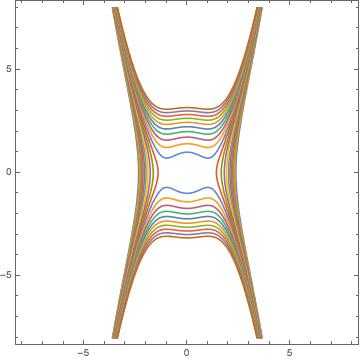
\includegraphics[width=.8\linewidth]{./ContourPlotB.jpeg}
      \caption*{eqns = Table[$\frac{y^2}{2} + \frac{x^2}{2} - \frac{x^4}{4} == n$, \{n, -100, 100, 2\}];}
      \caption*{ContourPlot[Evaluate@eqns, \{x, -8, 8\}, \{y, -8, 8\}]}
    \end{subfigure}%
    \begin{subfigure}{.5\textwidth}
      \centering
      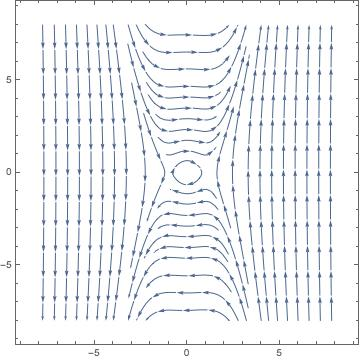
\includegraphics[width=.8\linewidth]{./StreamPlotB.jpeg}
      \caption*{StreamPlot[{$y$, $x^3 - x$}, {x, -8, 8}, {y, -8, 8}]}
    \end{subfigure}
    \end{figure}
    
    \begin{flushleft}
    There seem to be stable, homoclinic orbits that form circles near the origin as well as saddle, hetroclinic orbits that travel away from the origin through out this phase portrait.
    \end{flushleft}
    
    \newpage
    \item
    \begin{flushleft}
    $f(x) = \sin(x)$
    \newline
    
    $$F(x) = \int f(x)dx = -\cos(x)$$
    $$H(x,y) = \frac{y^2}{2} + F(x) = \frac{y^2}{2} -\cos(x) = C$$
    \end{flushleft}
    
    \begin{figure}[h]
    \centering
    \begin{subfigure}{.5\textwidth}
      \centering
      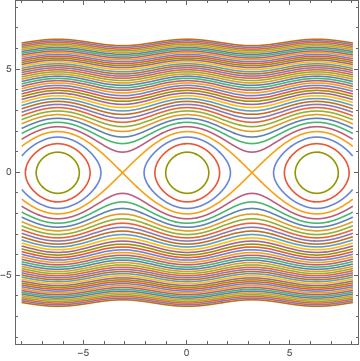
\includegraphics[width=.8\linewidth]{./ContourPlotC.jpeg}
      \caption*{eqns = Table[$\frac{y^2}{2} - Cos[x] == n$, \{n, -100, 100, 2\}];}
      \caption*{ContourPlot[Evaluate@eqns, \{x, -8, 8\}, \{y, -8, 8\}]}
    \end{subfigure}%
    \begin{subfigure}{.5\textwidth}
      \centering
      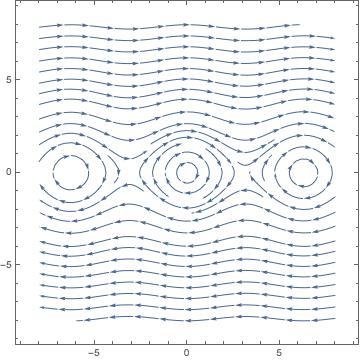
\includegraphics[width=.8\linewidth]{./StreamPlotC.jpeg}
      \caption*{StreamPlot[{y, -Sin[x]}, {x, -8, 8}, {y, -8, 8}]}
    \end{subfigure}
    \end{figure}
    
    \begin{flushleft}
    The types of orbits seen in this phase portrait include the periodic, saddle ones that seem to mirror the periodicity of the cosine function. There are also homoclinic orbits that form circles near the y(t) = 0 axis.
    \end{flushleft}
    
\end{enumerate} 
\end{flushleft}
\newpage
\item[(6)]
\begin{flushleft}
Determine the general solution of the system

$$\dot{x} = -y + \epsilon x(1 - x^2 - y^2)$$
$$\dot{y} = x + \epsilon y(1 - x^2 - y^2)$$

where $\epsilon$ is a real parameter.
\newline

By a change of variable to polar coordinates, we set $x(t) = r(t)\cos(\theta(t))$ and set $y(t) = r(t)\sin(\theta(t))$. By the properties of polar coordinates, we know that $r^2 = x^2 + y^2$ and $\theta = \tan^{-1}(\frac{y}{x})$. Differentiating both sides with respect to $t$, we get the following equations:
$$r\dot{r} = x\dot{x} + y\dot{y}$$
$$r^2\dot{\theta} = x\dot{y} - y\dot{x}$$
Solving for $\dot{r}$ and $\dot{\theta}$ and substituting our system of nonlinear equations gives us:
\begin{equation*}
\begin{split}\dot{r} & = \frac{x\dot{x} + y\dot{y}}{r} \\
& = \frac{x(-y + \epsilon x(1 - x^2 - y^2)) + y(x + \epsilon y(1 - x^2 - y^2))}{r} \\
& = \frac{-xy + \epsilon x^2(1 - x^2 - y^2) +yx + \epsilon y^2(1 - x^2 - y^2)}{r} \\
& = \frac{\epsilon (x^2 + y^2)(1 - x^2 - y^2)}{r} \\
& = \frac{\epsilon (r^2)(1 - (x^2 + y^2))}{r} \\
& = \epsilon r(1 - r^2) \\
& = \epsilon r - \epsilon r^3
\end{split}
\end{equation*}
We can then use the separation of variables method to solve the resulting ODE:
$$\frac{dr}{dt} = \epsilon r - \epsilon r^3$$
$$\frac{dr}{\epsilon r - \epsilon r^3} = dt$$
$$\int \frac{dr}{\epsilon r - \epsilon r^3} = \int dt = t$$
$$-\frac{ln(-r^2+1)}{2\epsilon} + \frac{ln(-r)}{\epsilon} = t + C$$
Using the laws of logarithms, we can simply the equation and since $r(t) > 0$ for polar coordinates, we get the positive solution:
$$r(t) = \frac{e^{\epsilon t}}{\sqrt{e^{2 \epsilon t}+ C}}$$
A similar analysis can be done for $\theta$:
\begin{equation*}
\begin{split}\dot{\theta} & = \frac{x\dot{y} - y\dot{x}}{r^2} \\
& = \frac{x(x + \epsilon y(1 - x^2 - y^2)) - y(-y + \epsilon x(1 - x^2 - y^2))}{r} \\
& = \frac{x^2 + \epsilon xy(1 - x^2 - y^2) + y^2 - \epsilon yx(1 - x^2 - y^2)}{r^2} \\
& = \frac{x^2 + y^2}{r^2} \\
& = 1
\end{split}
\end{equation*}
We can once again use the separation of variables method to solve the resulting ODE:
$$\frac{d\theta}{dt} = 1$$
$$d\theta = dt$$
$$\int d\theta = \int dt$$
$$\theta(t) = t + \theta_0$$
\vspace{.15in}
\begin{equation*}
\begin{split}
(x(t),y(t)) & = (r(t)\cos(\theta(t)), r(t)\sin(\theta(t))) \\
& = (\frac{e^{\epsilon t}}{\sqrt{e^{2 \epsilon t}+ C}}\cos(t + \theta_0), \frac{e^{\epsilon t}}{\sqrt{e^{2 \epsilon t}+ C}}\sin(t + \theta_0))
\end{split}
\end{equation*}
\end{flushleft}
\end{enumerate}
\end{document}